% !TeX root = ../../main.tex
\documentclass[../AAE590LGM_HW4.tex]{subfiles}
\begin{document}

\subsection{1.b)}
% Turning radius plot
\begin{figure}[H]
    \caption{Reference Trajectory}
    \centering
    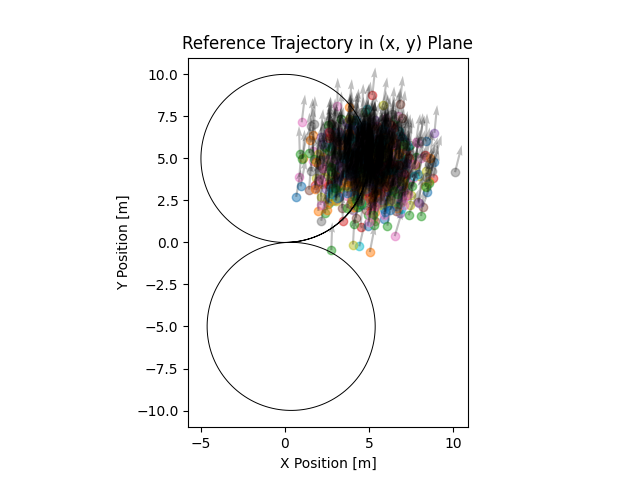
\includegraphics[width=0.7\linewidth]{AAE590LGM_HW4_Q1b_ref.png}
\end{figure}

\subsection{1.c)}
\begin{figure}[H]
    \caption{Gaussian Fit}
    \centering
    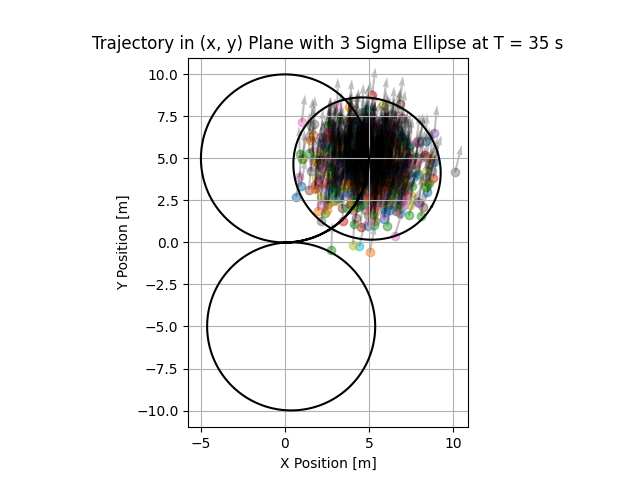
\includegraphics[width=0.7\linewidth]{AAE590LGM_HW4_Q1c_gfit.png}
\end{figure}

\subsection{1.e)}
\begin{figure}[H]
    \caption{Distribution at t = 5 s}
    \centering
    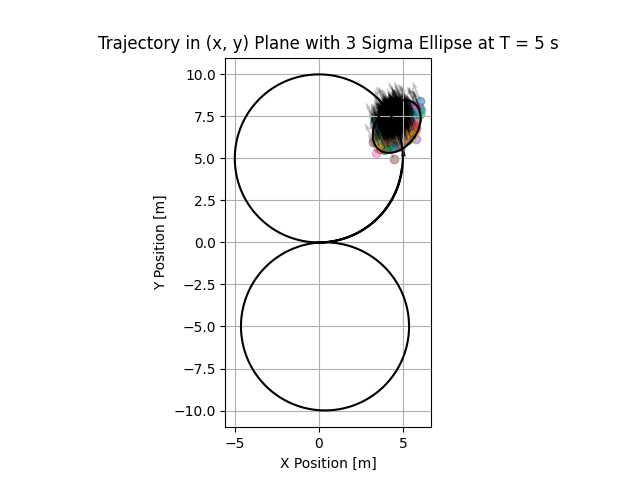
\includegraphics[width=0.7\linewidth]{AAE590LGM_HW4_Q1e_t5.png}
\end{figure}

\begin{figure}[H]
    \caption{Distribution at t = 15 s}
    \centering
    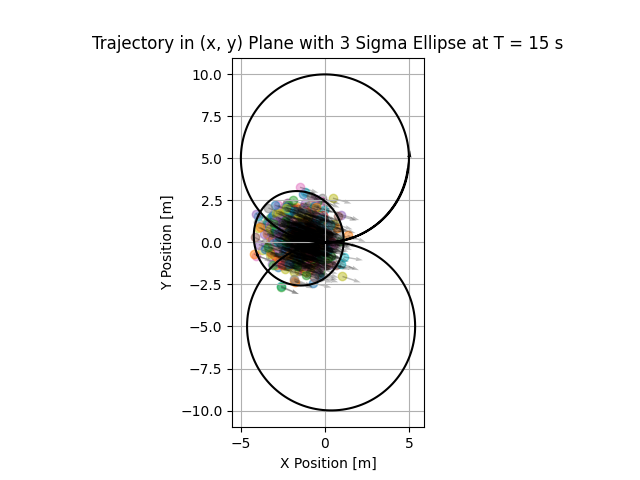
\includegraphics[width=0.7\linewidth]{AAE590LGM_HW4_Q1e_t15.png}
\end{figure}

\begin{figure}[H]
    \caption{Distribution at t = 30 s}
    \centering
    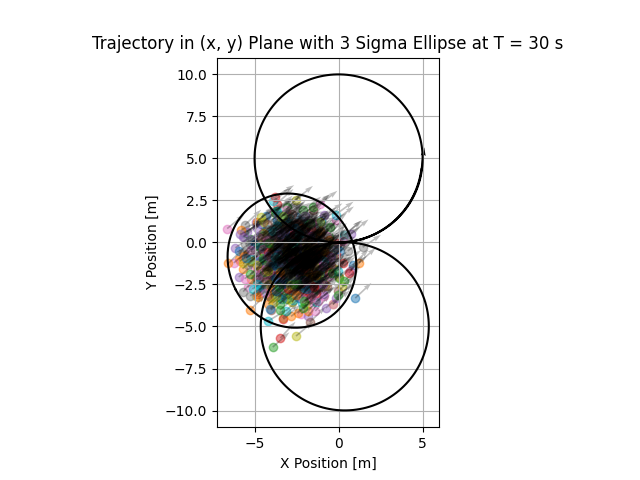
\includegraphics[width=0.7\linewidth]{AAE590LGM_HW4_Q1e_t30.png}
\end{figure}

\subsection{1.f)}
\begin{figure}[H]
    \caption{Distribution in Lie Algebra}
    \centering
    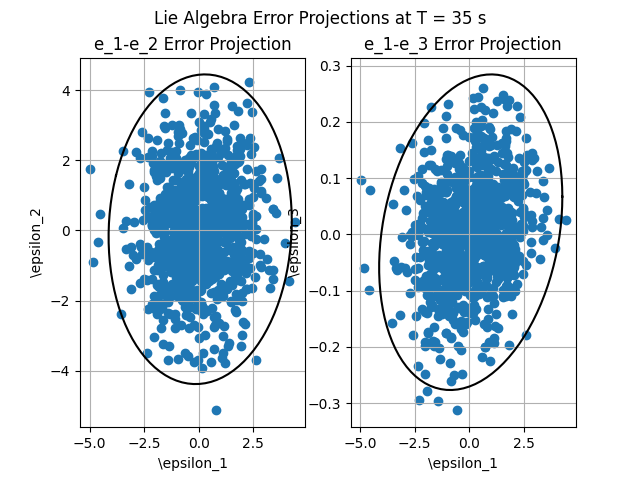
\includegraphics[width=0.7\linewidth]{AAE590LGM_HW4_Q1f_liealg.png}
\end{figure}

\subsection{1.g)}
\begin{figure}[H]
    \caption{Distribution at t = 35 s Projected from Lie Algebra}
    \centering
    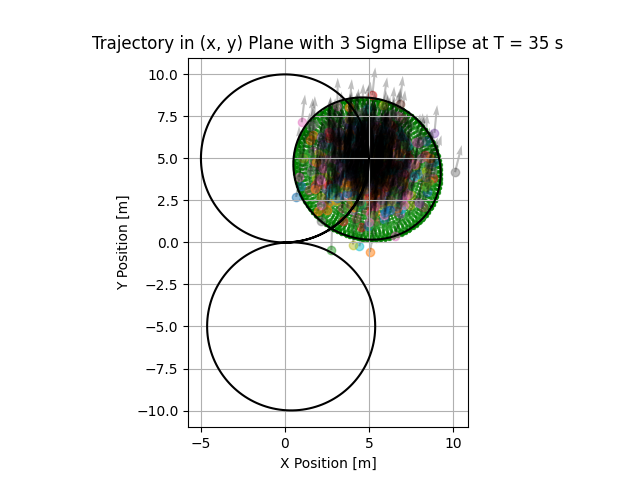
\includegraphics[width=0.7\linewidth]{AAE590LGM_HW4_Q1g_t35.png}
\end{figure}

% Code
\lstinputlisting[language=Python,caption={Problem Data Code, inputpath=../../../HW4}]{AAE590LGM_HW4_Problem.py}
\lstinputlisting[language=Python,caption={The Banana Distribution Code}]{AAE590LGM_HW4_Q1.py}


\end{document}
